% !Mode:: "TeX:UTF-8"
%%% Local Variables:
%%% mode: latex
%%% TeX-master: t
%%% End:

\chapter{基于生成对抗网络的遥感影像分割方法}
\label{cha:chap04}

\section{引言}
深度学习方法通过组合低阶特征形成更加抽象的高阶表示,基于全卷积架构的语义分割方法其多层的卷积网络结构可以完成对输入图像特征的自动学习。全卷积网络分割模型使用反卷积的上采样策略将特征图恢复到原始图像尺寸,完成对输入图像的像素级分类。然而,上采样过程造成了特征的损失,导致预测结果边界模糊的问题。另外,遥感影像由于其固有的信息不确定性,分类预测中地物边界模糊、歧义性等问题更加严重,全卷积语义分割方法在遥感影像分类中无法取得更佳的分类精度。
%同时,现有模型通常对每个像素类别进行预测,像素级别的准确率可能会很高,但是像素与像素之间的相关关系容易忽略,使得分割结果不够连续或者某个物体在分割结果中尺寸、形状与ground truth 图中的形状、尺寸差别较大。

生成对抗网络(Generative Adversarial Networks,GAN)训练时生成器(Genenrator)与判别器(Discriminator)不断对抗博弈,网络迭代好时判别器无法判断来源为生成器生成结果还是Ground truth 图,此时生成网络具有强大的图像生成能力\cite{luc2016semantic} 。本章将对抗网络应用到全卷积图像分割中,使得分割结果能够产生更好的地物边界,同类别物体空间上具有一致性。
%GAN 生成器生成原图的分割结果,GAN 判别器判断分割结果图来自Ground truth图还是生成器生成的语义分割结果。当判别器无法区分分割结果图的来源,ji


\section{基于生成对抗网络框架的影像分割方法}
\label{sec:firtst}

\subsection{生成对抗网络框架}
\label{sec:first-1}
GAN 是一种生成式的对抗网络,即通过对抗的方式,去学习数据分布的生成式模型。生成网络尽可能生成逼真样本,判别网络尽可能去辨别该样本是真实样本还是生成的假样本。

\begin{figure}[htb]
  \centering
  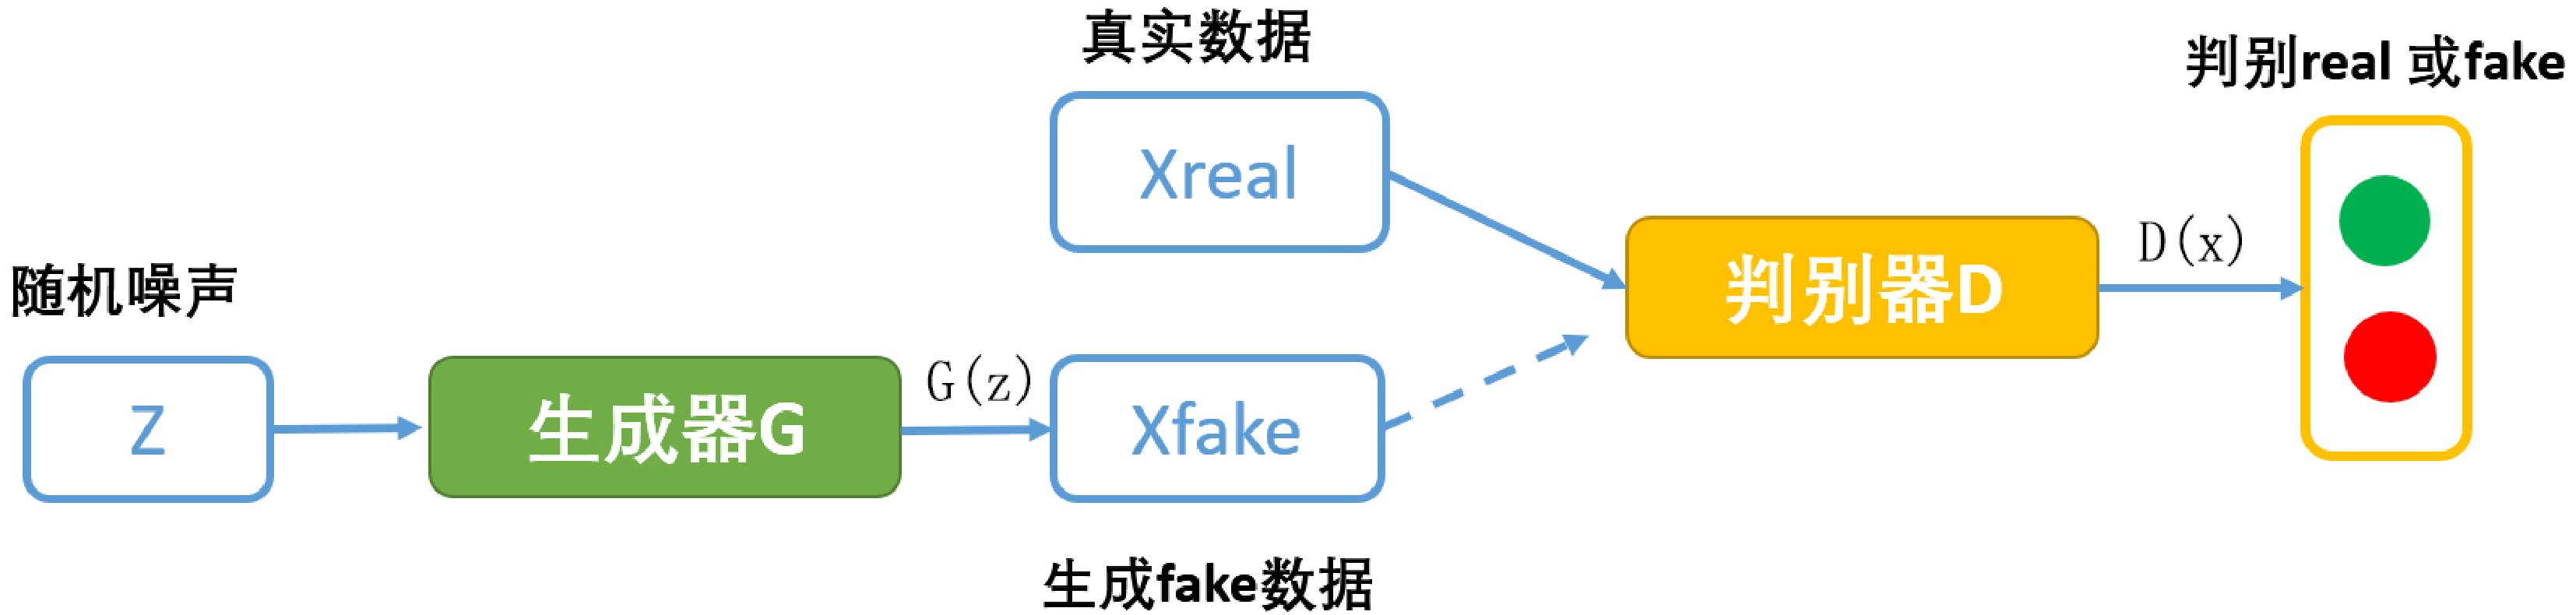
\includegraphics[width=0.8\textwidth]{figures/gan}
  \caption{GAN结构示意图}\label{fig:gan}
\end{figure}

如图\ref{fig:gan} 所示,假定变量$z$(通常为服从高斯分布的随机噪声)通过生成器G 生成$X_{fake}$,判别器D 负责判别输入的data 是生成的样本$X_{fake}$ 还是真实样本$X_{real}$。GAN 优化的目标函数为\ref{eq:4-1}:
\begin{equation}
  \label{eq:4-1}
  \mathop{\min}_{G} \mathop{\max}_{D} V(D,G) = \mathop{\min}_{G} \mathop{\max}_{D} E_{x \sim p_{data}(x)} [\log D(x)] + E_{z \sim p_{z}(z)}[ \log (1-D(G(z)))]
\end{equation}

式中$x \sim p_{data}(x)$ 表示$x$ 取自真实的分布数据。对于判别器D 来说,这是一个二分类问题,$ V(D,G)$ 为二分类中常见的交叉熵损失。对于生成器G 来说,为了尽可能欺骗D,需要最大化生成样本的判别概率$D(G(z))$ ,即最小化$\log (1-D(G(z)))$ 。

实际训练时,生成器G 和判别器D 采取交替训练,即先训练D ,再训练G ,不断往复。对于生成器G,最小化$\mathop{\max}_{D} V(D,G) $,即最小化$V(D,G)$ 的最大值。当生成器G 固定时,对$V(D,G)$ 求导,求出最优的判别器$D^{\star}(x)$:

\begin{equation}
  \label{eq:4-2}
  D^{\star}(x) = \frac{p_g(x)}{p_g(x)+p_{data}(x)}
\end{equation}

文献\cite{goodfellow2014generative} 中指出,当多次往复训练后,模型会收敛,G 与D 达到纳什均衡,此时$p_g(x) = p_{data}(x)$,即判别器对生成样本和真实样本的预测概率均为$\frac{1}{2}$, 无法区分。

传统的GAN 结构是无监督模型,只能生成真实的数据,不能生成我们想要的某一种类型的数据。文献\cite{mirza2014conditional} 提出条件生成对抗网络(Conditional Generative Adversarial Networks,CGAN),模型中加入条件约束$y$ 引导模型训练,生成我们需要的目标类型数据,$y$ 可以是任何种类的辅助信息,如样本标签,图像ground truth 图或其他不同领域模态的数据等。

\begin{figure}[htb]
  \centering
  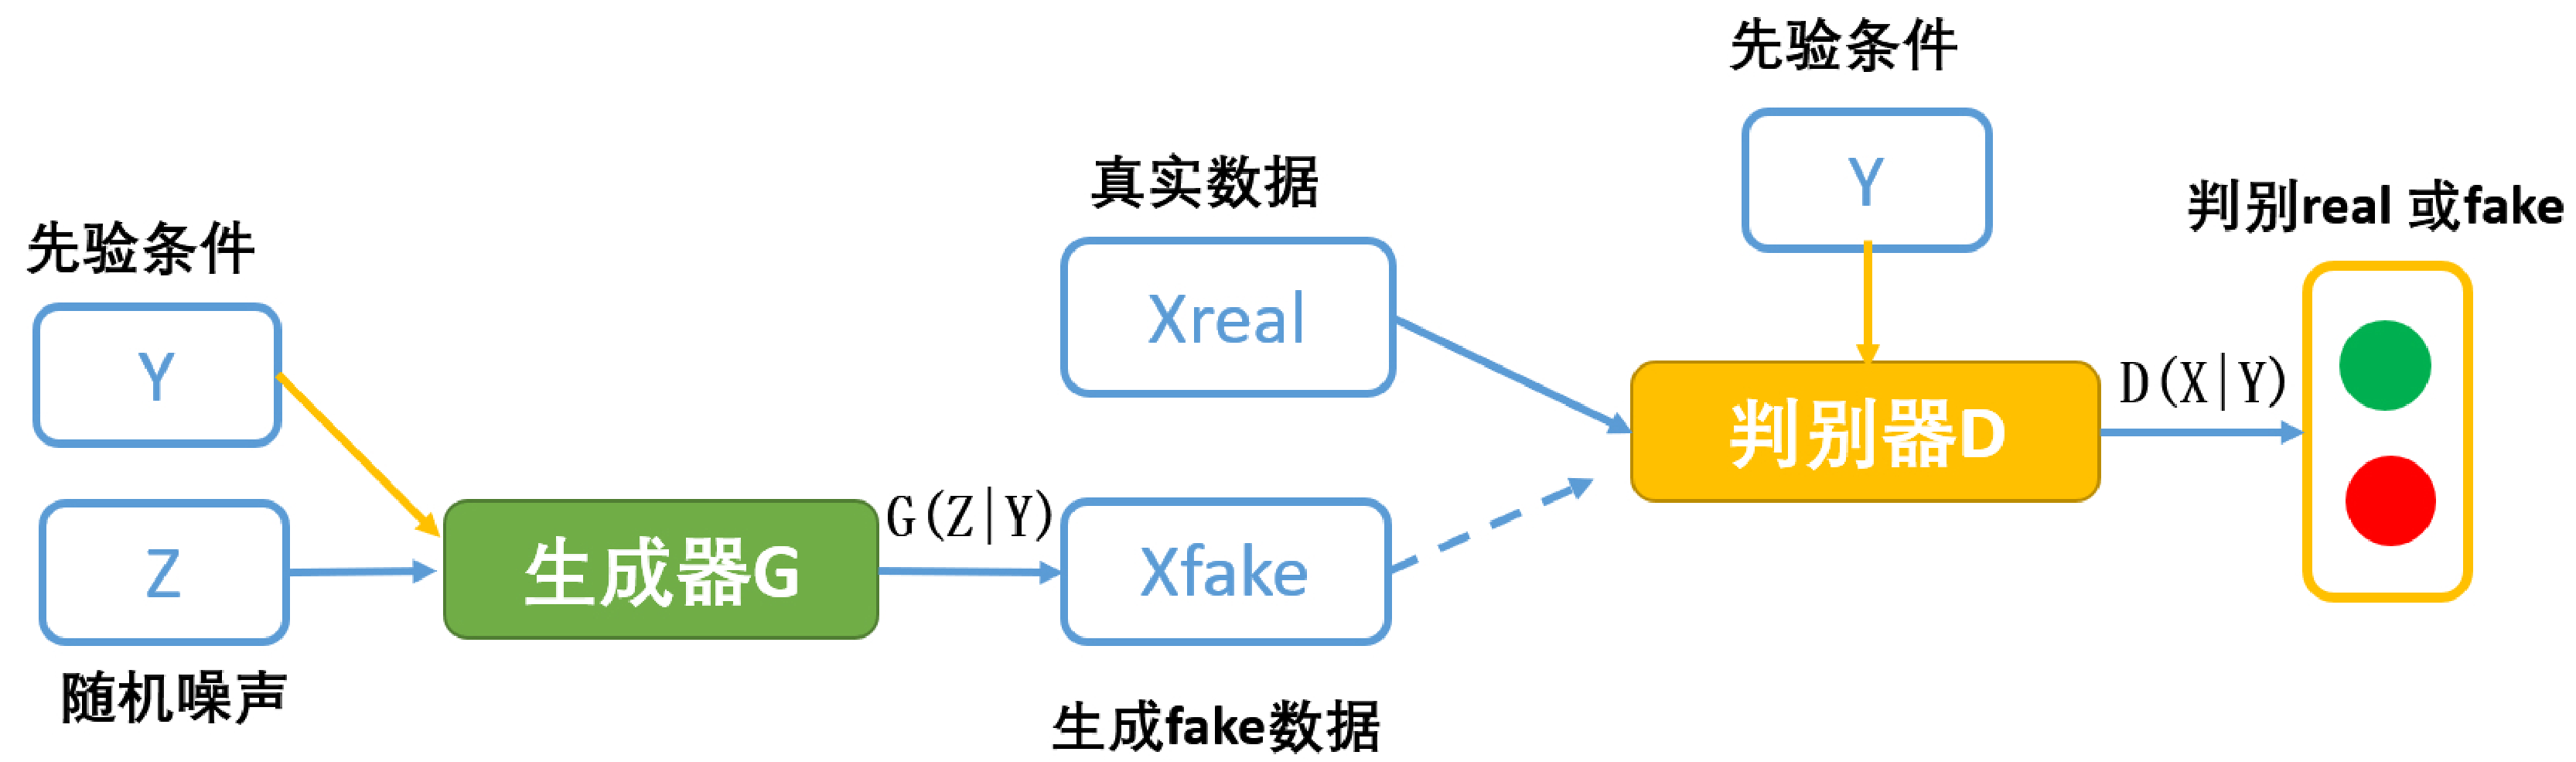
\includegraphics[width=0.8\textwidth]{figures/cgan}
  \caption{CGAN结构示意图}\label{fig:cgan}
\end{figure}

CGAN 模型中,生成器G 中随机噪声$z$与条件先验知识$y$ 被联合组成联合隐层输入特征;判别器D 中$X$ 和$y$ 通过词嵌入共同作为模型输入。 类似式\ref{eq:4-1}, CGAN 模型目标函数为带有条件概率的二人极小极大值博弈函数,即:

\begin{equation}
  \label{eq:4-3}
  \mathop{\min}_{G} \mathop{\max}_{D} V(D,G) = \mathop{\min}_{G} \mathop{\max}_{D} E_{x \sim p_{data}(x)} [\log D(x|y)] + E_{z \sim p_{z}(z)}[ \log (1-D(G(z|y)))]
\end{equation}

图\ref{fig:cgan} 为CGAN 的结构示意图,通过将额外条件信息$y$ 分别输送给判别模型和生成模型组成联合隐层表征,作为输入层的一部分,从而指导数据的生成过程。


\subsection{基于CGAN 的影像分割方法}
\label{sec:first-2}
基于图像条件的CGAN 影像分割方法主要包含两个阶段:生成网络的影像分割模型和对抗训练阶段的判别模型。整个方法处理流程如图\ref{fig:gan-fcn} 所示,左边生成网络是一个全卷积影像分割模型,右边对抗网络是一个二元分类判别模型。

\begin{figure}[htb]
  \centering
  \begin{center}
    \makebox[\textwidth]{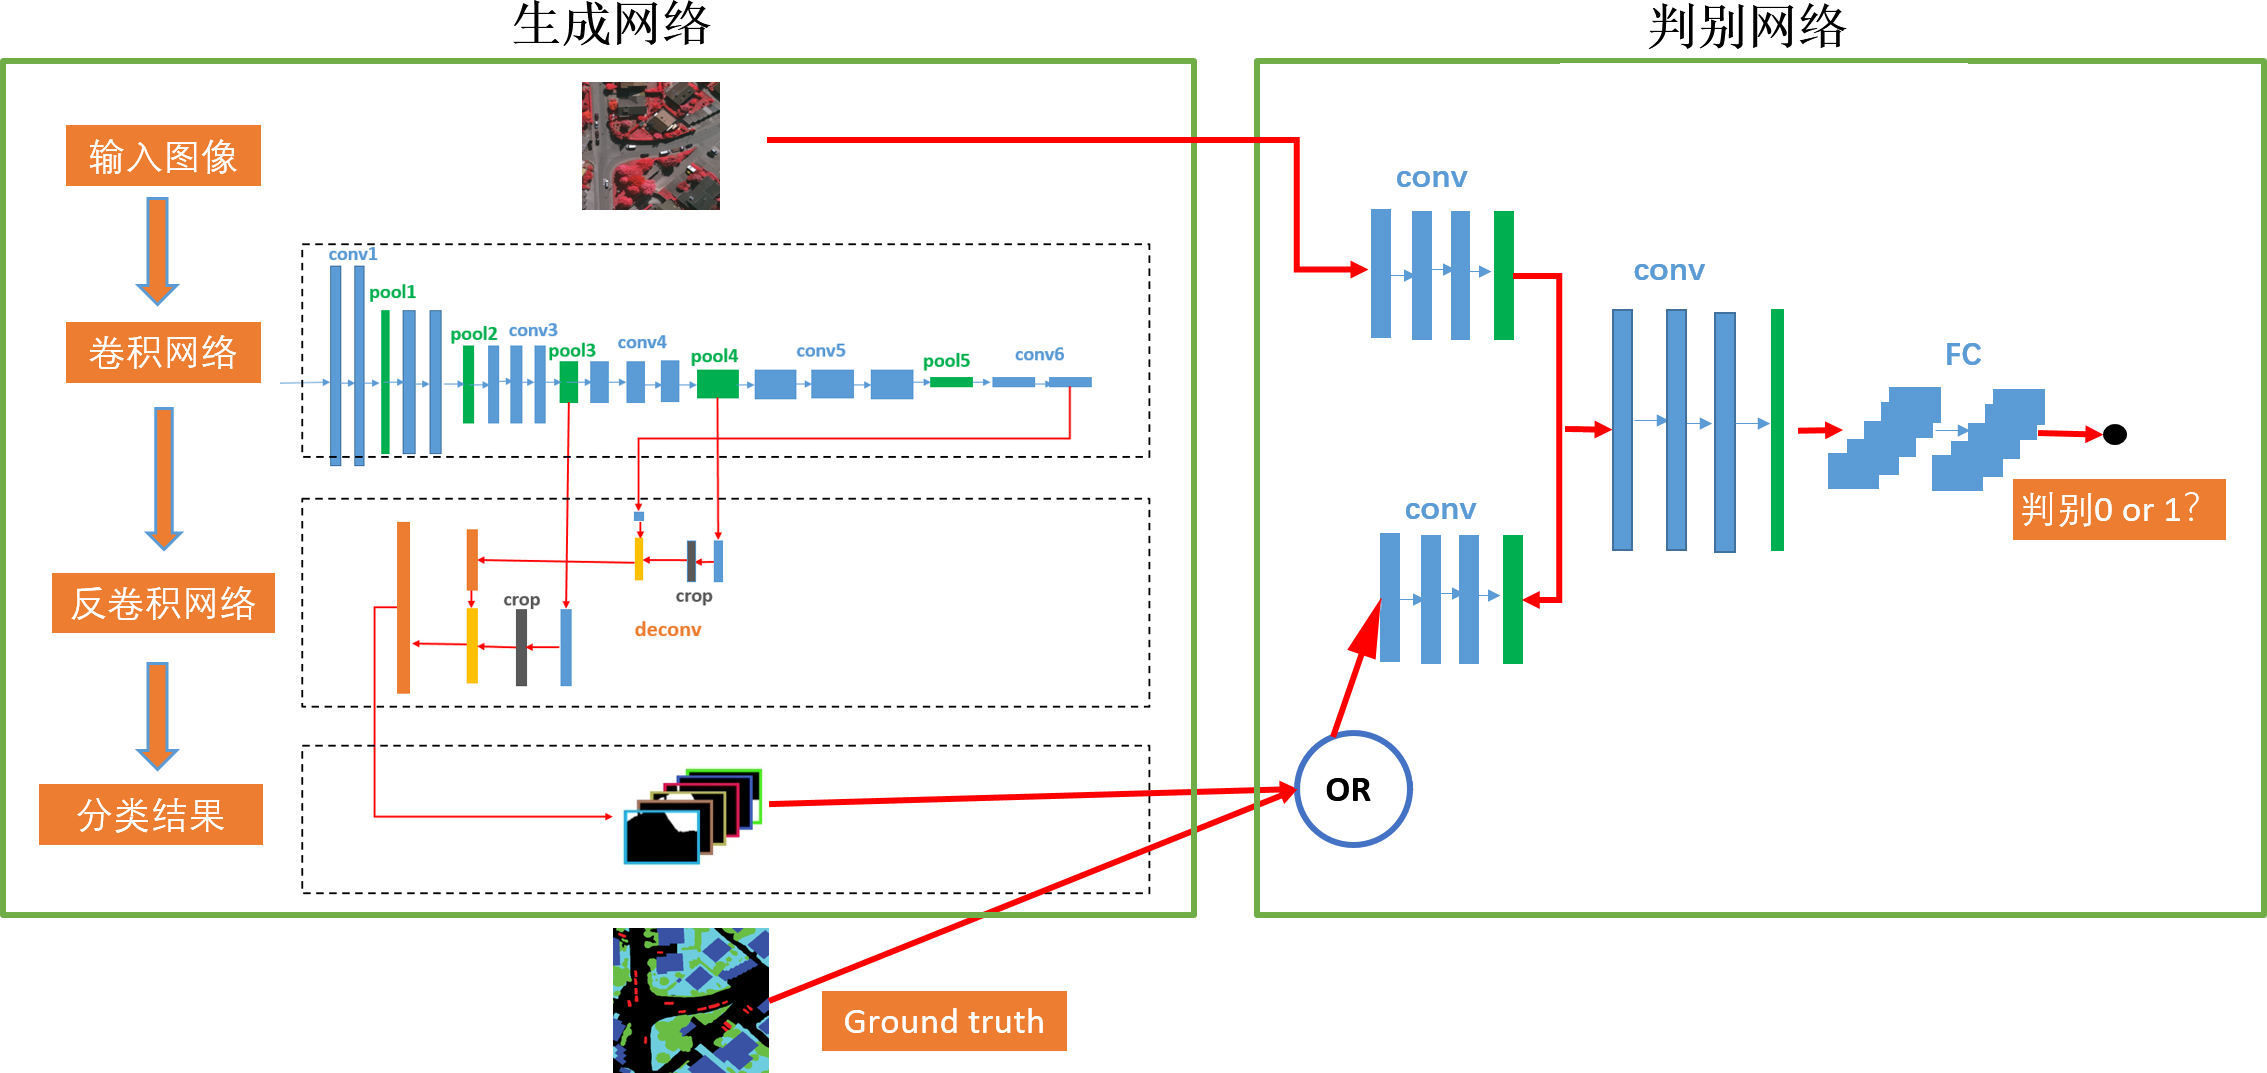
\includegraphics[width=\paperwidth]{figures/gan-fcn}}
    \caption{基于对抗训练框架的全卷积语义分割模型示意图}\label{fig:gan-fcn}
  \end{center}
\end{figure}

对抗网络的输入存在两种情况:一种是原始图像和ground truth 图拼接输入,另一种是原始图像与左边模型输出分割结果拼接输入。本文中对抗网络模型为一个六层卷积神经网络模型,一个卷积块由三个卷积层后接一个最大池化层组成,整个卷积网络由两个卷积块和两个全连接层堆叠形成。对抗网络的输出为一个二元分类值(输出为1代表它判断输入是第一种情况,输出为0代表它判断输入是第二种情况)。使用二元分类损失(Binary classification loss, BCE)来度量判别网络。二元分类损失为二元交叉熵(cross entropy)函数,统计学中使用KL 散度衡量两个事件或分布中的不同,常用于计算代价,而在特定任务下最小化KL散度等价于最小化交叉熵,而交叉熵的运算更简单\cite{de2005tutorial},所以这里用交叉熵来计算二元分类损失。交叉熵函数为分类预测概率值的负对数。二元交叉熵代价表达式如下:
\begin{equation}
  \label{eq:4-4}
  l_{bce} (\hat{z}, z) = -[z\log\hat{z} + (1-z)\log(1-\hat{z})]
\end{equation}

%+ (1-y_{ic})\log(1-\hat{y}_{ic})
生成网络是全卷积网络模型,其是一个多分类网络模型。经典的多分类分割模型代价函数为多类别的交叉熵损失(multi-class entropy loss, MCE),则分割模型输入为大小为$H\times W\times C$ 的图像,对图像做像素级预测分类,其多元交叉熵损失为:
\begin{equation}
  \label{eq:4-5}
  l_{mce} (\hat{y}, y) = -\sum_{i=1}^{H\times W}\sum_{c=1}^{C}y_{ic}\log\hat{y}_{ic}
\end{equation}
其中,$H$、$W$ 和$C$ 分别为图像的高度、宽度以及通道数。假定多分类问题中类标有$K$ 个取值,需要使用独热编码(One-hot encode)将图像类别标签编码为一个$K$ 维向量,借助Softmax 函数作为分类任务的输出层。Softmax 函数把神经网络分类输出转化为一组概率,且这组概率和为1。归属于类别$j$ 的概率为:%softmax(z_j) = 
\begin{equation}
  \label{eq:4-6}
  p_j = \frac{e^{z_j}}{\sum_{k=1}^Ke^{z_k}}  \quad \forall j \in 1,2,\cdots, K
\end{equation}

假定有$N$ 张训练图片的数据集$X = \{x_1,x_2,\cdots, x_n \}$,对应的ground truth 图标签集为$Y = \{y_1,y_2,\cdots, y_n \}$。输入图像大小为$H\times W\times C$(一般$C$ 取$3$),有$K$ 个类别的图像标签编码为$K$  维向量,即对第$i$ 张图像$x_i$,对应ground truth 图有$y_j = [y_j^{(1)},y_j^{(2)}, \cdots, y_j^{(K)}]$。我们定义$g(x)$ 为输入图片$x$ 在生成网络分割模型下的预测输出,定义$d(x,y)\in [0,1]$ 为对抗网络判别图像标签$y$ 是输入图像$x$ 对应的ground truth 图还是分割模型产生的分割结果的概率输出值。基于条件对抗网络框架的全卷积语义分割模型方法需要最小化分割模型的多分类交叉熵损失,同时最大化分割模型生成样本的判别概率。优化的目标代价函数为式\ref{eq:4-7}:
\begin{equation}
  \label{eq:4-7}
  L(\theta_g,\theta_d) = \sum_{n=1}^N \lbrace l_{mce} (g(x_n),y(n)) - \lambda [l_{bce} (d(x_n,y_n),1) + l_{bce}(d(x_n,g(x_n)),0)] \rbrace
\end{equation}
式中$\theta_g$ 和$\theta_d$ 分别代表分割模型和判别模型网络参数,右式中第一项为分割模型的交叉熵损失,第二项为对抗网络中样本判别损失代价函数,$\lambda$ 为生成阶段与对抗阶段代价权衡常数且有$\lambda > 0$。模型训练时我们需要最小化式\ref{eq:4-7} 中的代价函数,从而迭代求解得到网络参数$\theta_g$ 和$\theta_d$。

当模型迭代收敛后,模型中的权值参数均得以确定,此时模型中生成网络部分已经具有优秀的图像分割识别能力。通过前向传播,利用最终分割模型对待分类测试影像求解每个像素属于各个类别的概率值,像素点所属类别概率值求采用式\ref{eq:4-6} 中Softmax 函数求解,再利用argmax 函数求出最大概率值对应类别标签维度,即为当前像素的类别标签,影像$x$ 上任一像素点$i$ 所属类别标签$C_k$ 的计算方式如式\ref{eq:4-8}。
\begin{equation}
  \label{eq:4-8}
  C_k = \mathop{\arg\max}_{k \in K} p_k(x^{(i)}), \ k=1,2,\cdots,K
\end{equation}
类似地,对测试影像所有像素点求出类别标签,即可实现测试影像的语义分割。


\section{实验数据介绍}
\label{sec:second}

\subsection{Vaihingen 数据介绍}
\label{sec:second-1}
本章实验数据源为ISPRS(国际摄影测量及遥感探测学会)提供的Vaihingen 高分辨率遥感影像数据\footnote{Vaihingen 数据集官网链接:http://www2.isprs.org/commissions/comm3/wg4/detection-and-reconstruction.html}。Vaihingen 数据集由德国测量和遥感协会(DGRF)于2010年使用空中数字摄像机拍摄,拍摄区域为半农村地区的德国斯图加特市法伊欣根市镇(Vaihingen),影像空间分辨率为$0.09m$。如图\ref{fig:vaihingen}(a) 所示为Vaihingen 数据整体图,整个数据被划分为33幅大小不一的图像,其中带有真实地面数据的影像为16幅。Vaihingen 数据包含三个波段(近红外-红-绿)的正射影像数据(Orthophoto)、数字地表模型(Digital Surface Model,DSM)数据以及拍摄区域真实地物分类结果(Ground truth)。图\ref{fig:vaihingen}(b-d) 为影像数据某一区域的正射影像及其DSM、真实地物分类结果。

\begin{figure}[htb]
  \centering
  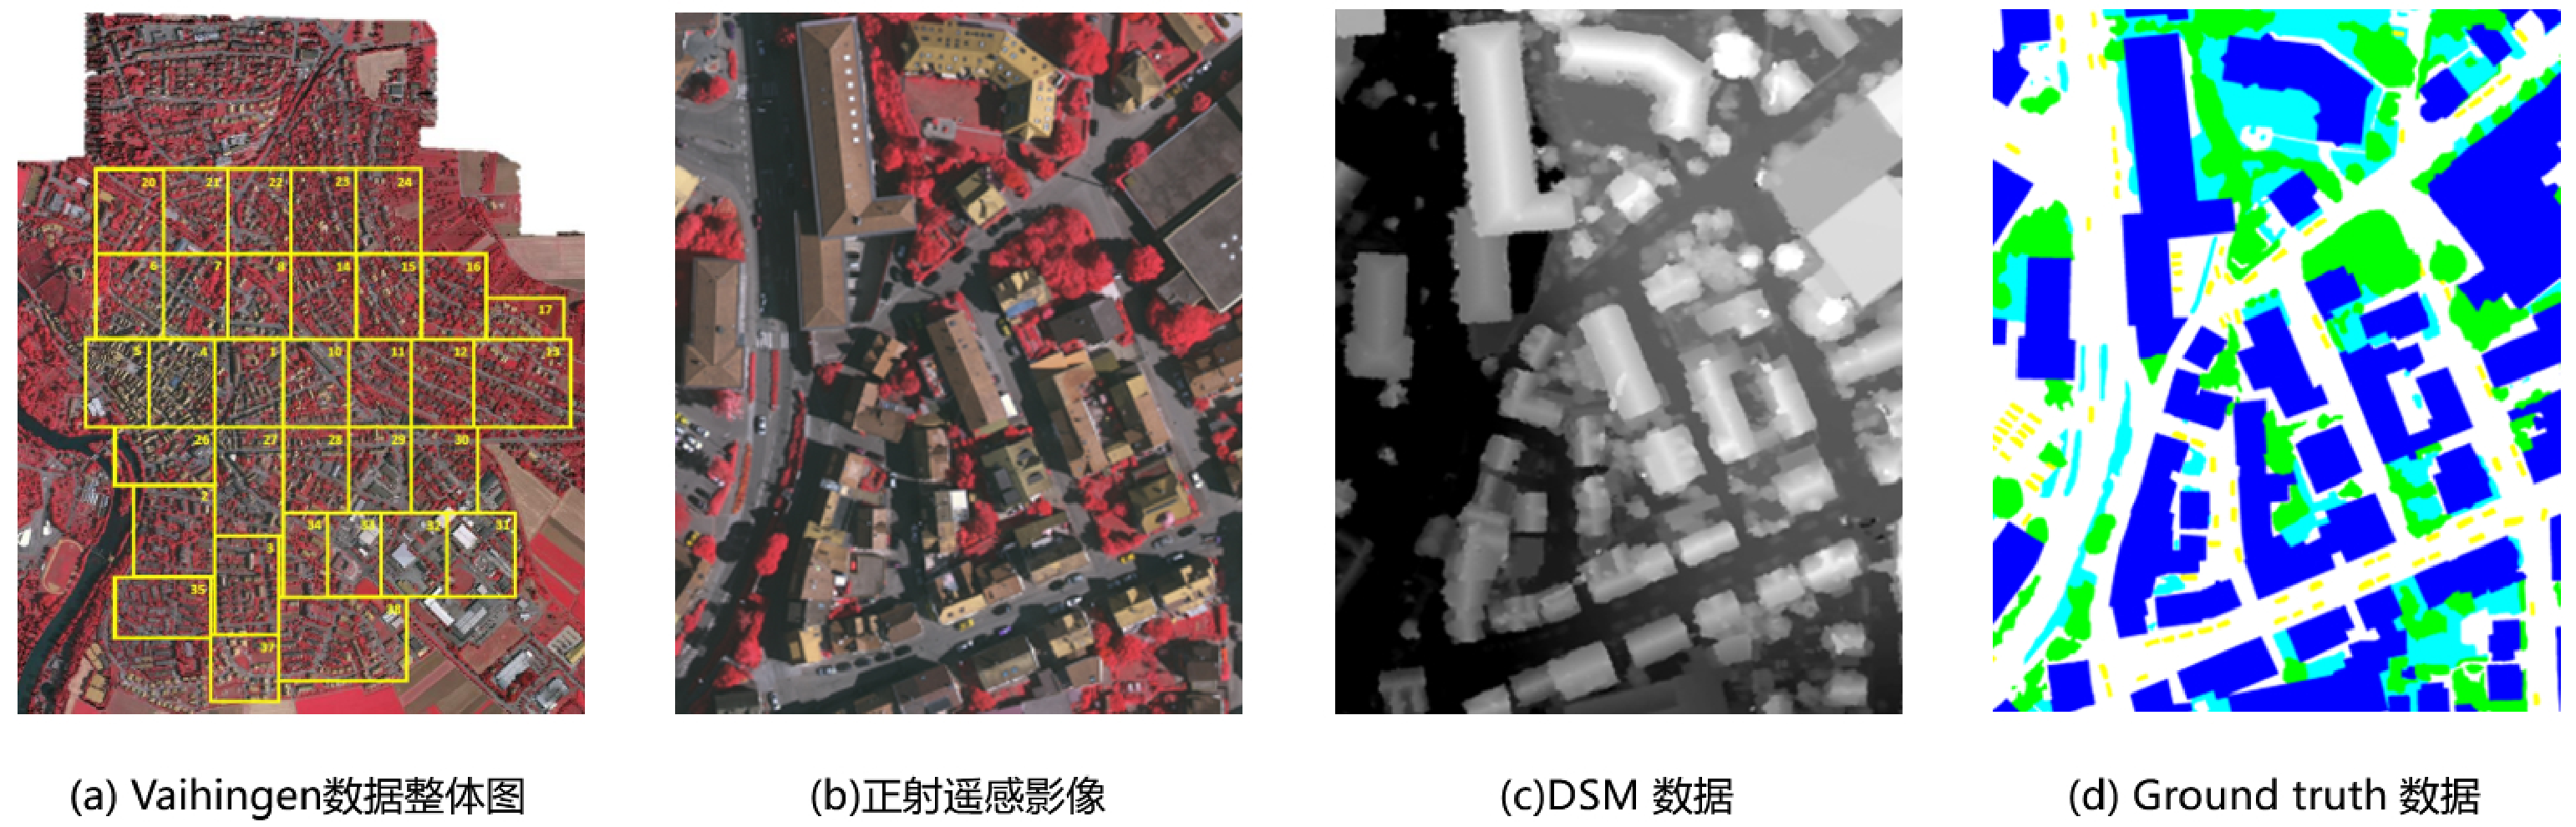
\includegraphics[width=0.98\textwidth]{figures/vaihingen2}
  \caption{Vaihingen 影像数据}\label{fig:vaihingen}
\end{figure}

Vaihingen 地区影像依据领域专家人工解译结果划分为地面、低矮植被、树木、建筑物、车辆、背景六类地物。Ground truth 图中六类地物的类别和对应颜色分别如表\ref{tab:vaih_gt} 所示。

\begin{table}[htbp]
  \caption{Vaihingen 数据类别标签颜色对照表}\label{tab:vaih_gt}
  \centering
  \footnotesize

  \begin{tabular}{p{2cm}p{2cm}p{3cm}p{2cm}}
    \toprule
    地物类别 & 颜色 & 色彩值(R,G,B)   & 类别标签 \\
    \midrule
    地面     & 白色 & $(255,255,255)$ & 0        \\
    低矮植被 & 青色 & $(0,255,255)$   & 1        \\
    树木     & 绿色 & $(0,255,0)$     & 2        \\
    建筑物   & 蓝色 & $(0,0,255) $    & 3        \\
    车辆     & 黄色 & $(255,255,0)$   & 4        \\
    背景     & 红色 & $(255,0,0) $    & 5        \\
    \bottomrule
  \end{tabular}
\end{table}

\subsection{数据预处理}
\label{sec:second-1}

\subsubsection*{1. 波段组合}
Vaihingen 高分辨率影像空间、几何信息丰富,但正射影像光谱波段只有三个,仅使用正射影像数据无法完备有效地提取影像特征。而对于光谱相似区域的地物,如地面、建筑物、阴影等,更加难以区分,DSM 数据是包含了地表建筑物、桥梁和树木等高度的地面高程模型,对模型区分地表建筑物、地面影像、不同高度植被一定程度上能提供帮助。Vaihingen 影像的DSM 包含一个波段,其像素值表示高度值。因此,将Vaihingen 数据的DSM 作为额外的波段附加在正射影像波段后,参与模型训练。

\subsubsection*{2. 数据集划分}
Vaihingen 数据中带有Ground truth 图影像共有16张,实验中选取12张影像(标号为$1,5,7,11,15,17,21,26,28,30,32$ 和$37$)作为模型训练集,另外4张影像(标号为$3,13,23,34$)作为模型测试集。

\subsection{实验数据准备}
\label{sec:second-1}

本章实验数据源为ISPRS


\section{实验结果与分析}
\label{sec:third}
(国际摄影测量及遥感探测学会)提供的


\section{本章小结}
\label{sec:forth}
(国际摄影测量及遥感探测学会)提供的